% -*- latex -*-
%%%%%%%%%%%%%%%%%%%%%%%%%%%%%%%%%%%%%%%%%%%%%%%%%%%%%%%%%%%%%%%%
%%%%%%%%%%%%%%%%%%%%%%%%%%%%%%%%%%%%%%%%%%%%%%%%%%%%%%%%%%%%%%%%
%%%%
%%%% This text file is part of the source of 
%%%% `Parallel Programming in MPI and OpenMP'
%%%% by Victor Eijkhout, copyright 2012-2021
%%%%
%%%% hybrid.tex : about hybrid computing
%%%%
%%%%%%%%%%%%%%%%%%%%%%%%%%%%%%%%%%%%%%%%%%%%%%%%%%%%%%%%%%%%%%%%
%%%%%%%%%%%%%%%%%%%%%%%%%%%%%%%%%%%%%%%%%%%%%%%%%%%%%%%%%%%%%%%%

So far, you have learned to use MPI for distributed memory and OpenMP
for shared memory parallel programming. However, distribute memory
architectures actually have a shared memory component, since each
cluster node is typically of a multicore design. Accordingly, you
could program your cluster using MPI for inter-node and OpenMP for
intra-node parallelism.

You now have to find the right balance between processes and threads,
since each can keep a core fully busy.
Complicating this story, a node can have more than one \indexterm{socket},
and corresponding \indexac{NUMA} domain.
%
\begin{figure}[ht]
  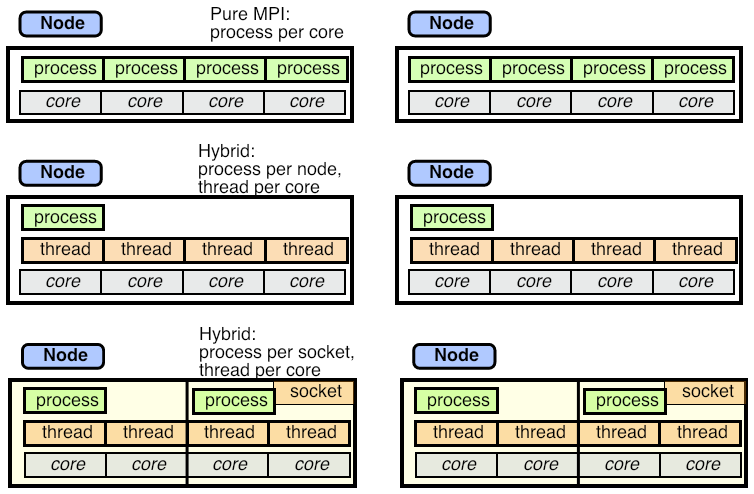
\includegraphics[scale=.5]{mpi-omp-hybrid}
  \caption{Three modes of MPI/OpenMP usage on a multi-core cluster}
  \label{fig:hybrid-modes}
\end{figure}
%
Figure~\ref{fig:hybrid-modes} illustrates three modes: pure MPI
with no threads used; one MPI process per node and full
multi-threading; two MPI processes per node, one per socket, and
multiple threads on each socket.

\Level 0 {Affinity}

\index{affinity!process and thread|(}

In the preceeding chapters we mostly considered all MPI nodes or
OpenMP thread as being in one flat pool.
However, for high performance you need to worry about \indextermdef{affinity}:
the question of which process or thread is placed where, and how
efficiently they can interact.

\begin{figure}[ht]
  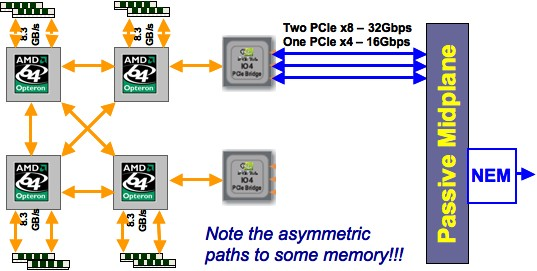
\includegraphics[scale=.7]{ranger-numa}
  \caption{The NUMA structure of a Ranger node}
  \label{fig:ranger-numa}
\end{figure}

Here are some situations where you affinity becomes a concern.
\begin{itemize}
\item In pure MPI mode processes that are on the same node can
  typically communicate faster than processes on different
  nodes. Since processes are typically placed sequentially, this means
  that a scheme where process~$p$ interacts mostly with $p+1$ will be
  efficient, while communication with large jumps will be less so.
\item If the cluster network has a structure
  (\indextermsub{processor}{grid} as opposed to \indexterm{fat-tree}),
  placement of processes has an effect on program efficiency.  MPI
  tries to address this with \indexterm{graph topology};
  section~\ref{sec:mpi-dist-graph}.
\item Even on a single node there can be
  asymmetries. Figure~\ref{fig:ranger-numa} illustrates the structure
  of the four sockets of the \indexterm{Ranger} supercomputer (no
  longer in production). Two cores have no direct connection.

  This asymmetry affects both MPI processes and threads on that node.
\item Another problem with multi-socket designs is that each socket
  has memory attached to it. While every socket can address all the
  memory on the node, its local memory is faster to access. This
  asymmetry becomes quite visible in the \indexterm{first-touch}
  phenomemon; section~\ref{sec:first-touch}.
\item If a node has fewer MPI processes than there are cores, you want
  to be in control of their placement. Also, the operating system can
  migrate processes, which is detrimental to performance since it
  negates data locality. For this reason, utilities such as
  \indextermtt{numactl}
\begin{tacc}
(and at TACC \indextermtt{tacc_affinity})    
\end{tacc}
  can be used to \indexterm{pin a thread} or process to a specific core.
\item Processors with \indexterm{hyperthreading} or
  \indextermsub{hardware}{threads} introduce another level or worry
  about where threads go.
\end{itemize}

\Level 0 {What does the hardware look like?}

If you want to optimize affinity, you should first know what the
hardware looks like. The \indextermttdef{hwloc} utility is valuable
here~\cite{goglin:hwloc} (\url{https://www.open-mpi.org/projects/hwloc/}).

\begin{figure}[ht]
  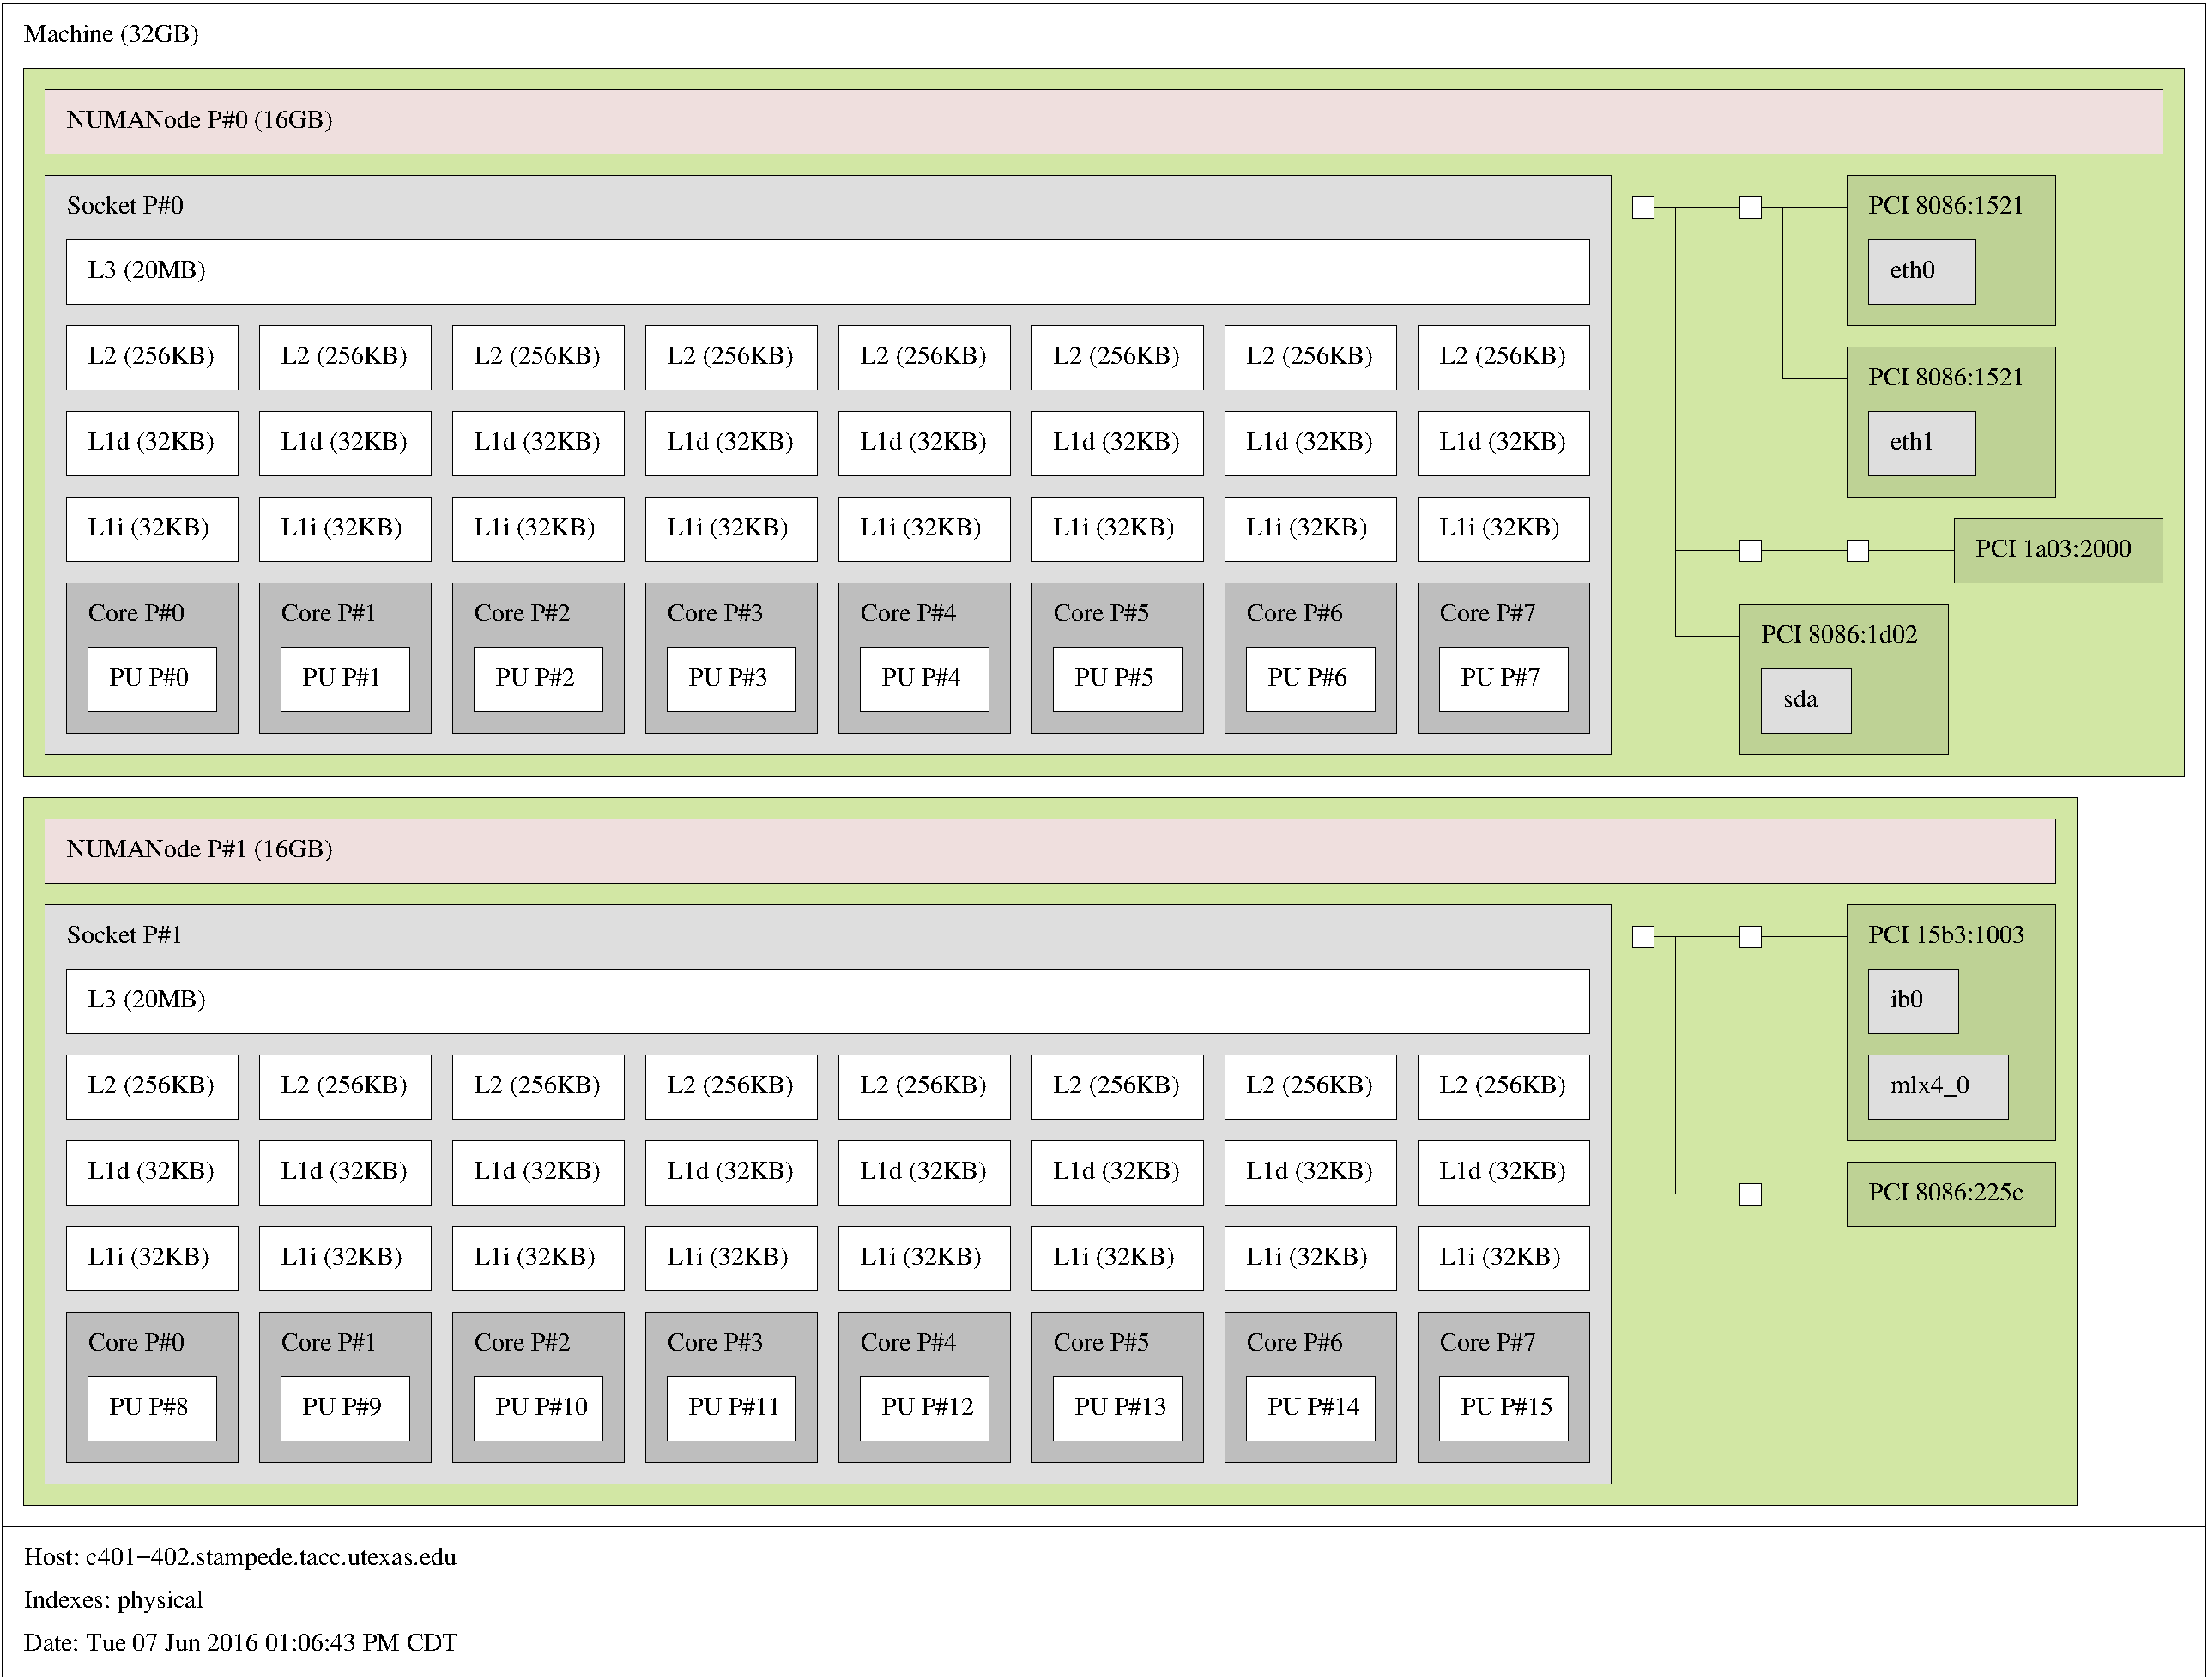
\includegraphics[scale=.3]{stampede-compute}
  \caption{Structure of a Stampede compute node}
  \label{fig:stampede-compute-hwloc}
\end{figure}

\begin{figure}[p]
  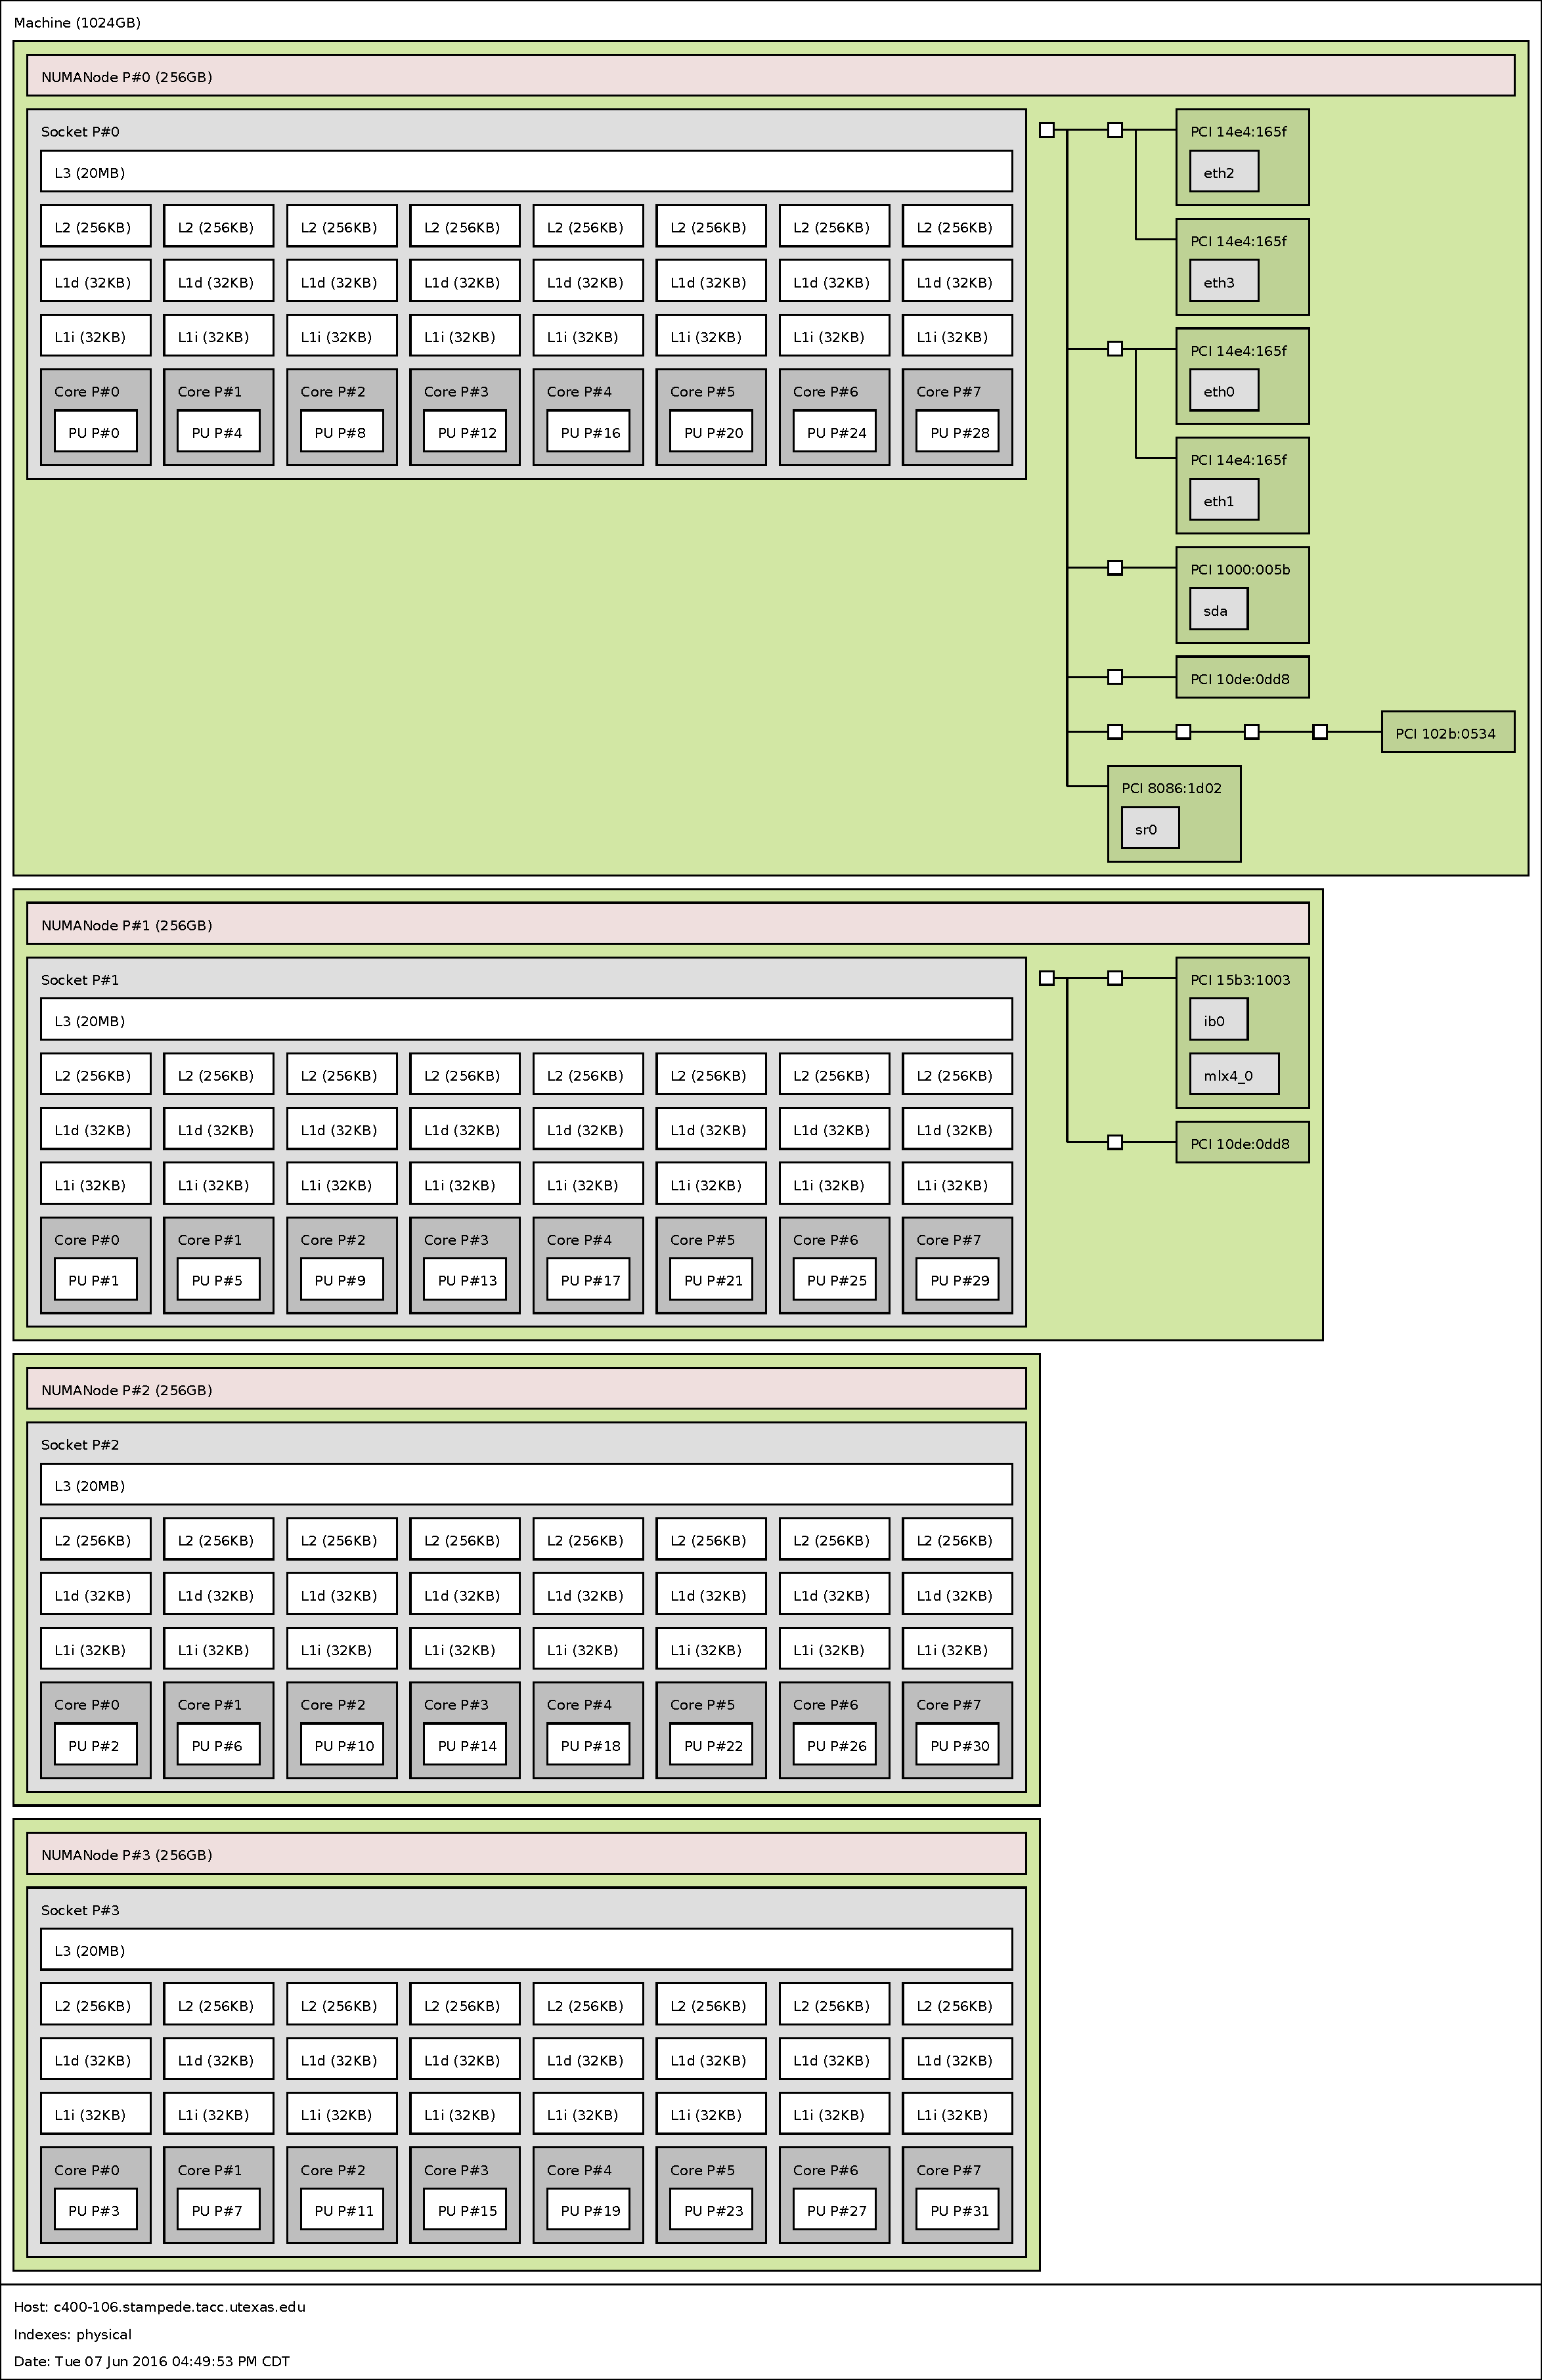
\includegraphics[scale=.3]{stampede-largemem}
  \caption{Structure of a Stampede largemem four-socket compute node}
  \label{fig:stampede-largemem-hwloc}
\end{figure}

\begin{figure}[ht]
  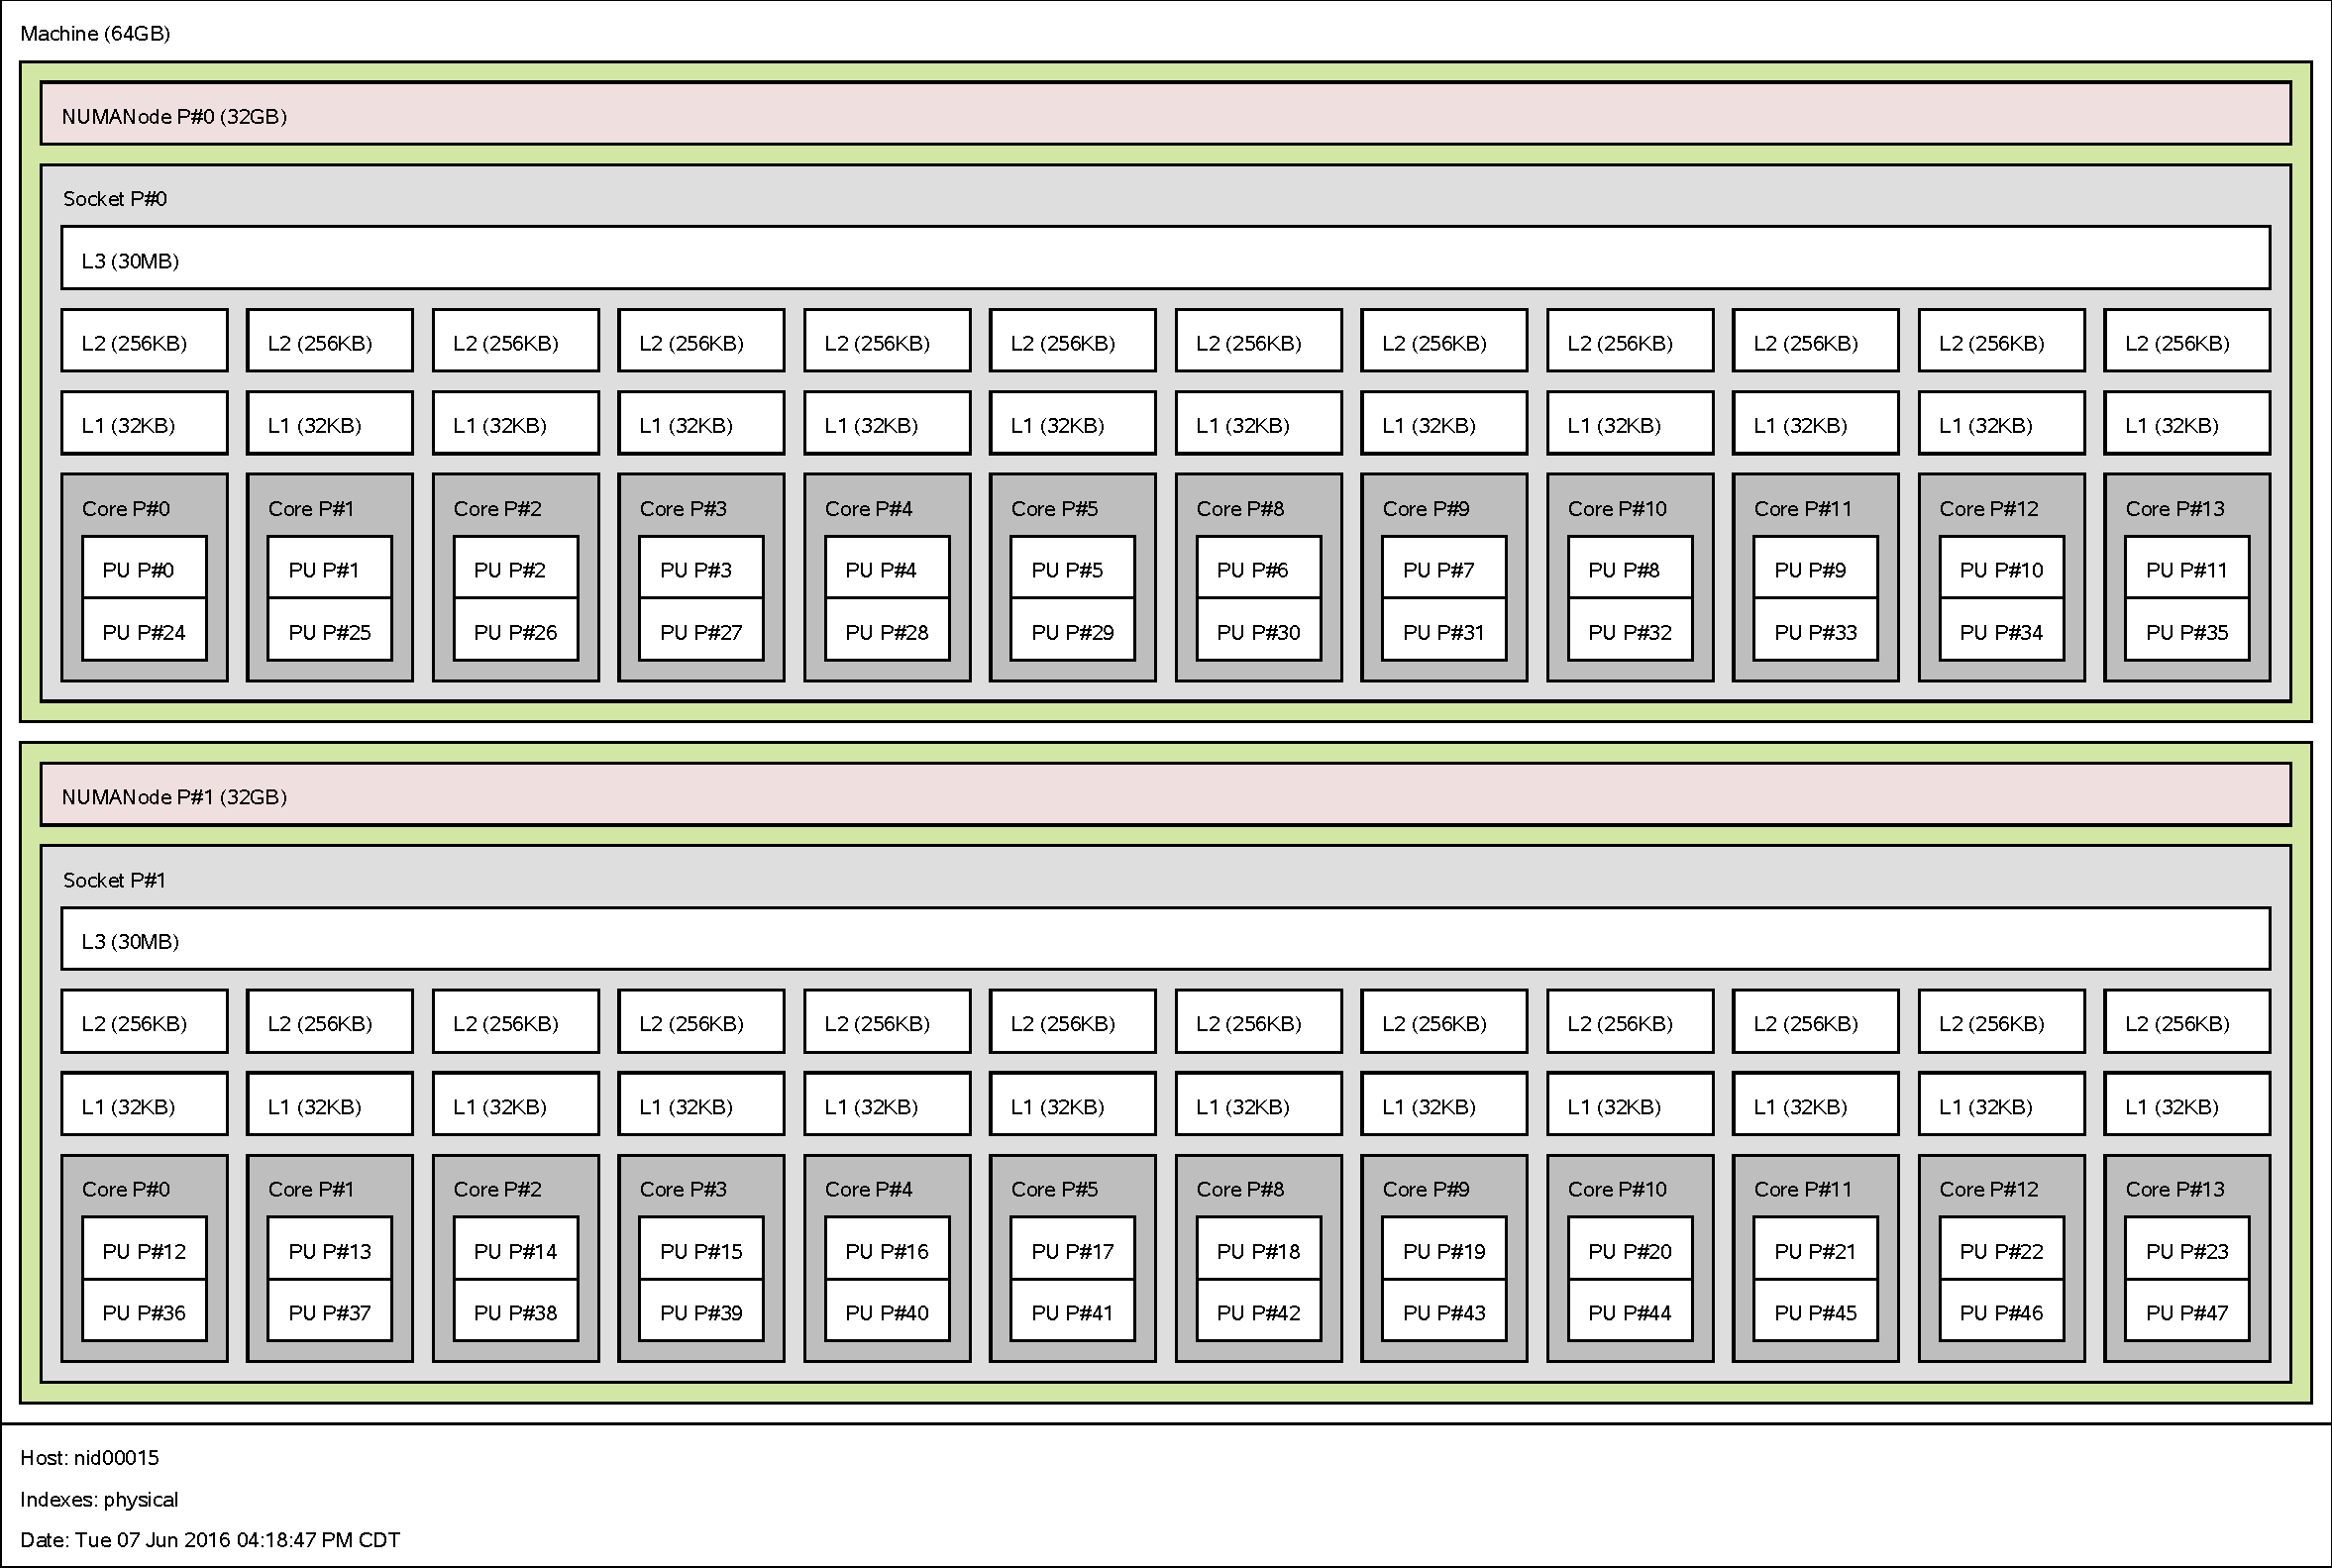
\includegraphics[scale=.3]{ls5}
  \caption{Structure of a Lonestar5 compute node}
  \label{fig:ls5-compute-hwloc}
\end{figure}

Figure~\ref{fig:stampede-compute-hwloc} depicts a
\indextermbus{Stampede}{compute node}, which is a two-socket
\indextermbus{Intel}{Sandybridge} design;
figure~\ref{fig:stampede-largemem-hwloc} shows a 
\indextermbus{Stampede}{largemem node}, which is a four-socket design.
%
Finally, figure~\ref{fig:ls5-compute-hwloc} shows a
\indexterm{Lonestar5} compute node, a~two-socket design with 12-core
\indextermbus{Intel}{Haswell} processors with two hardware threads
each.

\Level 0 {Affinity control}

See chapter~\ref{ch:omp-affinity} for OpenMP affinity control.

\index{affinity!process and thread|)}

\Level 0 {Discussion}

The performance implications of the pure MPI strategy versus hybrid
are subtle.
\begin{itemize}
\item First of all, we note that there is no obvious speedup: in a
  well balanced MPI application all cores are busy all the time, so
  using threading can give no immediate improvement.
\item Both MPI and OpenMP are subject to Amdahl's law that quantifies
  the influence of sequential code; in hybrid computing there is a new
  version of this law regarding the amount of code that is
  MPI-parallel, but not OpenMP-parallel.
\item MPI processes run unsynchronized, so small variations in load or
  in processor behavior can be tolerated. The frequent barriers in
  OpenMP constructs make a hybrid code more tightly synchronized, so
  load balancing becomes more critical.
\item On the other hand, in OpenMP codes it is easier to divide the
  work into more tasks than there are threads, so statistically a
  certain amount of load balancing happens automatically.
\item Each MPI process has its own buffers, so hybrid takes less
  buffer overhead.
\end{itemize}

\begin{exercise}
  Review the scalability argument for 1D versus 2D matrix
  decomposition in \HPSCref{sec:parallel-dense-mvp}. Would you get
  scalable performance from doing a 1D decomposition (for instance, of
  the rows) over MPI processes, and decomposing the other directions
  (the columns) over OpenMP threads?
\end{exercise}

Another performance argument we need to consider concerns message
traffic.  If let all threads make MPI calls (see
section~\ref{sec:init-thread}) there is going to be little
difference. However, in one popular hybrid computing strategy we would
keep MPI calls out of the OpenMP regions and have them in effect done
by the master thread.
%
In that case there are only MPI messages
between nodes, instead of between cores. This leads to a decrease in
message traffic, though this is hard to quantify. The number of
messages goes down approximately by the number of cores per node, so
this is an advantage if the average message size is small. On the
other hand, the amount of data sent is only reduced if there is
overlap in content between the messages.

Limiting MPI traffic to the master thread also means that no buffer
space is needed for the on-node communication.

\Level 0 {Hybrid MPI-plus-threads execution}
\label{sec:init-thread}
\label{sec:ref:mpi-thread}

While the MPI standard itself makes no mention of threads
--~process being the primary unit of computation~--
the use of threads is allowed.
Below we will discuss what provisions exist for doing so.

Using threads and other shared memory models in combination with MPI
leads of course to the question how
\indexterm{race condition}s are handled.
Example of a code with a data race that pertains to MPI:
\begin{lstlisting}
#pragma omp sections
#pragma omp section
  MPI_Send( x, /* to process 2 */ )
#pragma omp section
  MPI_Recv( x, /* from process 3 */ )
\end{lstlisting}
The MPI standard here puts the burden on the user:
this code is not legal, and behavior is not defined.

\Level 1 {MPI support for threading}

In hybrid execution, the main question is whether all threads
are allowed to make MPI calls. To determine this,
replace the \n{MPI_Init} call by
%
\indexmpiref{MPI_Init_thread}
%
Here the \n{required} and \n{provided} parameters can take the following
(monotonically increasing) values:
\begin{itemize}
\item \indexmpidef{MPI_THREAD_SINGLE}: Only a single thread will
  execute.
\item\indexmpidef{MPI_THREAD_FUNNELED}: The program may use multiple
  threads, but only the main thread will make MPI calls.

    The main thread is usually the one selected by the
    \indexpragma{master} directive, but technically it is the only that
    executes \indexmpishow{MPI_Init_thread}. If you call this routine in
    a parallel region, the main thread may be different from the master.
\item\indexmpidef{MPI_THREAD_SERIALIZED}: The program may use multiple
  threads, all of which may make MPI calls, but there will never be
  simultaneous MPI calls in more than one thread.
\item\indexmpidef{MPI_THREAD_MULTIPLE}: Multiple threads may issue MPI
  calls, without restrictions.
\end{itemize}

After the initialization call, you can query the support level
with \indexmpiref{MPI_Query_thread}.

In case more than one thread performs communication, 
\indexmpiref{MPI_Is_thread_main}
can determine whether a thread is the main thread.

\begin{mplnote}{Threading support}
  \ac{MPL} always calls \indexmpishow{MPI_Init_thread}
  requesting the highest level \indexmpishow{MPI_THREAD_MULTIPLE}.
\begin{lstlisting}
enum mpl::threading_modes {
  mpl::threading_modes::single = MPI_THREAD_SINGLE, 
  mpl::threading_modes::funneled = MPI_THREAD_FUNNELED,
  mpl::threading_modes::serialized = MPI_THREAD_SERIALIZED,
  mpl::threading_modes::multiple = MPI_THREAD_MULTIPLE
};
threading_modes mpl::environment::threading_mode ();
bool mpl::environment::is_thread_main ();
\end{lstlisting}
\end{mplnote}

\begin{tacc}
  The \indexterm{mvapich} implementation of MPI
  does have the required threading support, but you need to set this environment variable:  
\begin{verbatim}
export MV2_ENABLE_AFFINITY=0
\end{verbatim}
  Another solution is to run your code like this:
\begin{verbatim}
  ibrun tacc_affinity <my_multithreaded_mpi_executable
\end{verbatim}
  Intel MPI uses an environment variable to turn on thread support:
\begin{verbatim}
I_MPI_LIBRARY_KIND=<value>
where
release : multi-threaded with global lock
release_mt : multi-threaded with per-object lock for thread-split  
\end{verbatim}
\end{tacc}

The \emph{mpiexec}\index{mpiexec!and environment variables}
program usually propagates \indexterm{environment variables},
so the value of \indextermtt{OMP_NUM_THREADS} when you call \n{mpiexec}
will be seen by each MPI process.

\begin{itemize}
\item It is possible to use blocking sends in threads, and let the
  threads block. This does away with the need for polling.
\item You can not send to a thread number: use the MPI
  \indextermbus{message}{tag} to send to a specific thread.
\end{itemize}

\begin{exercise}
Consider the 2D heat equation and explore the mix of MPI/OpenMP
parallelism:
\begin{itemize}
\item Give each node one MPI process that is fully multi-threaded.
\item Give each core an MPI process and don't use multi-threading.
\end{itemize}
Discuss theoretically why the former can give higher performance.
Implement both schemes as special cases of the general hybrid case,
and run tests to find the optimal mix.
\end{exercise}

\cverbatimsnippet[examples/mpi/c/thread.c]{thread}

\Level 0 {Processes and cores and affinity}

In OpenMP, threads are purely a software construct and you can create
however many you want.
The hardware limit of the available cores can be queried with
\indexompshow{omp_get_num_procs} (section~\ref{sec:omp-howmany}).
How does that work in a hybrid context?
Does the `proc' count return the total number of cores,
or does the MPI scheduler limit it to a number exclusive to each MPI process?

The following code fragment explore this:

\cverbatimsnippet[examples/hybrid/c/procthread.c]{corecountttotal}

Running this with \indextermbus{Intel}{MPI} (version~19)
gives the following:
\begin{verbatim}
---- nprocs: 14
Omp procs on this process: 4
Omp procs total: 56
---- nprocs: 15
Omp procs on this process: 3
Omp procs total: 45
---- nprocs: 16
Omp procs on this process: 3
Omp procs total: 48
\end{verbatim}
We see that
\begin{itemize}
\item Each process get an equal number of cores, and
\item Some cores will go unused.
\end{itemize}

While the OpenMP `proc' count is such that the MPI processes will not
oversubscribe cores, the actual placement of processes and threads
is not expressed here.
This assignment is known as \indexterm{affinity} and it is
determined by the MPI/OpenMP runtime system.
Typically it can be controlled through environment variables,
but one hopes the default assignment makes sense.
\begin{figure}[ht]
  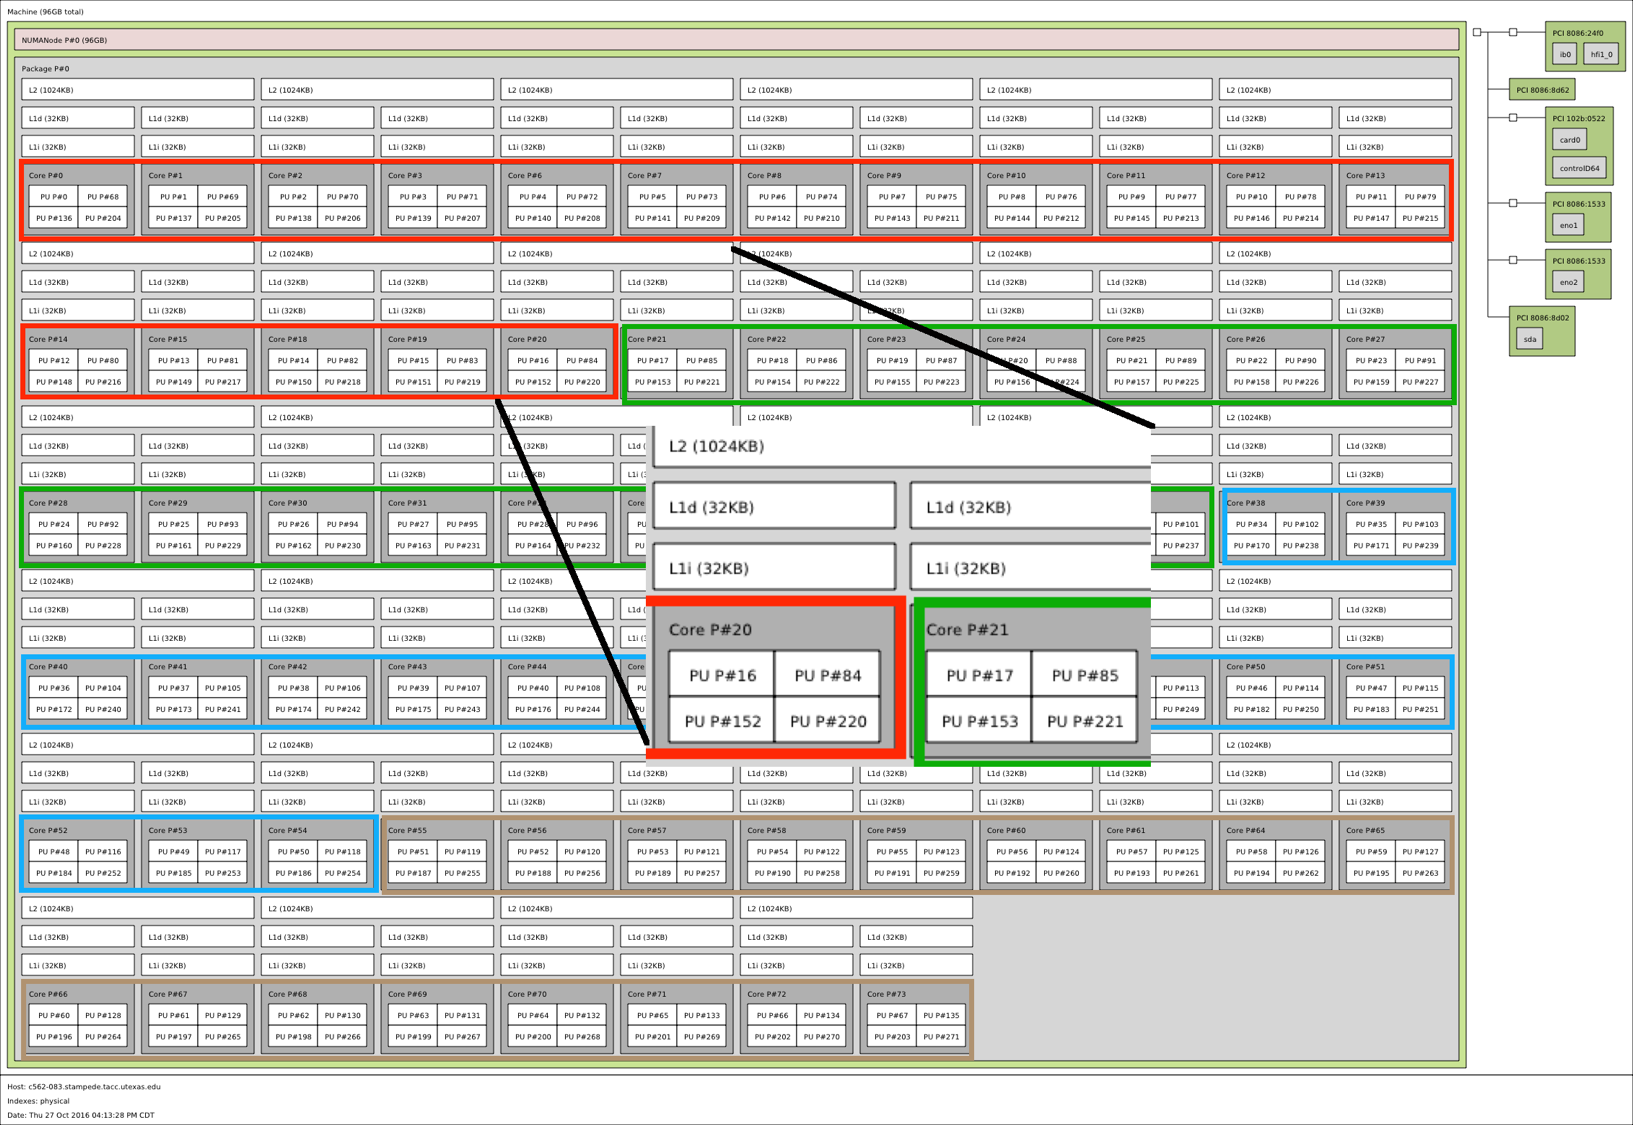
\includegraphics[scale=.5]{knl-affinity}
  \caption{Process and thread placement on an Intel Knights Landing}
  \label{fig:knl-affinity}
\end{figure}
Figure~\ref{fig:knl-affinity} illustrates this for the
\indextermbus{Intel}{Knights Landing}:
\begin{itemize}
\item Placing four MPI processes on 68 cores gives 17 cores per process.
\item Each process receives a contiguous set of cores.
\item However, cores are grouped in `tiles' of two, so processes 1~and~3 start
  halfway a tile.
\item Therefore, thread zero of that process is bound to the second core.
\end{itemize}

\Level 0 {Practical specification}

Say you use 100 cluster nodes, each with 16 cores. You could then
start 1600 MPI processes, one for each core, but you could also start
100 processes, and give each access to 16 OpenMP threads.

\begin{tacc}
In your slurm scripts, the first scenario would be specified \n{-N 100
-n 1600}, and the second as
\begin{verbatim}
#$ SBATCH -N 100
#$ SBATCH -n 100

export OMP_NUM_THREADS=16
\end{verbatim}
\end{tacc}

There is a third choice, in between these extremes, that makes
sense. A~cluster node often has more than one socket, so you could put
one MPI process on each \indexterm{socket}, and use a number of
threads equal to the number of cores per socket.

\begin{tacc}
The script for this would be:
\begin{verbatim}
#$ SBATCH -N 100
#$ SBATCH -n 200

export OMP_NUM_THREADS=8
ibrun tacc_affinity yourprogram
\end{verbatim}

The \indextermtt{tacc_affinity} script unsets the following variables:
\begin{verbatim}
export MV2_USE_AFFINITY=0
export MV2_ENABLE_AFFINITY=0
export VIADEV_USE_AFFINITY=0
export VIADEV_ENABLE_AFFINITY=0
\end{verbatim}
If you don't use \n{tacc_affinity} you may want to do this by hand,
otherwise \indexterm{mvapich2} will use its own affinity rules.
\end{tacc}
